\section{Capítulo 1 -- Como a Web funciona}

Antes de escrever a primeira linha de HTML, vale entender o caminho que uma página percorre até aparecer na tela: quem a guarda, como ela é pedida, como chega e o que o navegador faz com ela. Neste capítulo você vai conhecer a diferença entre a Internet e a Web, o modelo cliente-servidor, as partes de um endereço, o DNS, o protocolo HTTP e as etapas que o navegador percorre para desenhar uma página. No final, você vai preparar as ferramentas de trabalho e criar a primeira página, com um arquivo de HTML, um de CSS e um de JavaScript.

\subsection{1.1 Internet e Web}

As duas palavras costumam ser usadas como sinônimos, mas não são a mesma coisa. A \textbf{Internet} é a rede: milhões de computadores do mundo inteiro ligados por cabos, fibras e antenas, que trocam dados seguindo um conjunto de regras comum, os protocolos TCP/IP. Ela existe desde os anos 1970 e carrega muitos serviços diferentes: e-mail, mensagens, chamadas de vídeo, jogos.

A \textbf{Web} (\textit{World Wide Web}) é um desses serviços: um conjunto de documentos, as \textbf{páginas}, que ficam guardados em computadores espalhados pela Internet e são ligados uns aos outros por \textbf{links}. Ela foi proposta em 1989 por Tim Berners-Lee, um pesquisador do CERN, o laboratório europeu de física de partículas, para que os cientistas compartilhassem documentos. Em 1991, ele publicou o primeiro site, junto com as três peças que sustentam a Web até hoje:

\begin{itemize}
  \item o \textbf{HTML}, a linguagem em que as páginas são escritas;
  \item a \textbf{URL}, o endereço único de cada página;
  \item o \textbf{HTTP}, o protocolo que o navegador usa para pedir uma página e o servidor usa para entregá-la.
\end{itemize}

As regras dessas tecnologias são definidas por organizações abertas. O \textbf{WHATWG}, formado pelas empresas que fazem os navegadores, mantém o HTML como um \textbf{padrão vivo} (\textit{living standard}): não existe mais uma versão ``final'', e o padrão é atualizado continuamente. O nome HTML5, ainda muito usado, se refere à grande atualização publicada em 2014 e virou sinônimo de ``HTML moderno''. O \textbf{W3C} mantém o CSS e outros padrões. Para consultar como cada recurso funciona, a referência mais usada é o \textbf{MDN Web Docs} (\texttt{developer.mozilla.org}), mantido pela Mozilla, com tradução para o português em boa parte das páginas.

\subsection{1.2 Cliente e servidor}

Toda visita a um site envolve dois papéis. O \textbf{cliente} é quem pede: no caso da Web, o \textbf{navegador}, como o Chrome, o Firefox, o Edge ou o Safari. O \textbf{servidor} é um computador, ligado o tempo todo à Internet, que guarda os arquivos do site e os entrega a quem pedir. A conversa entre os dois é sempre a mesma: o cliente faz um \textbf{pedido} (a \textbf{requisição}) e o servidor devolve uma \textbf{resposta}.

\begin{center}
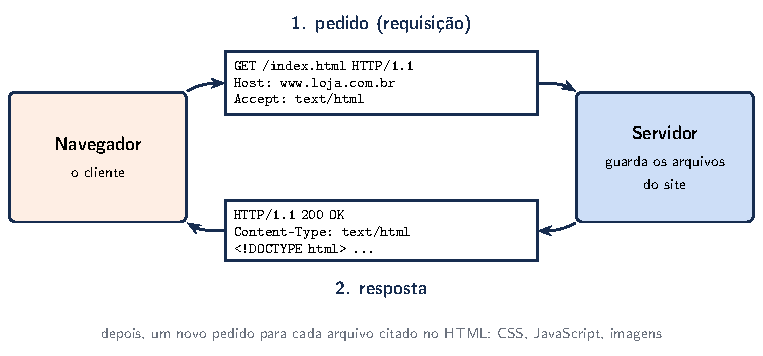
\includegraphics[width=0.95\linewidth,keepaspectratio]{imagens/capitulo-01_requisicao.pdf}
\end{center}

Uma página quase nunca é um arquivo só. O HTML cita outros arquivos, como folhas de estilo, \textit{scripts} e imagens, e o navegador faz um novo pedido para cada um deles, um atrás do outro ou vários ao mesmo tempo. Uma página de um grande portal chega a fazer centenas de pedidos até ficar pronta.

O servidor pode entregar dois tipos de conteúdo. Um site \textbf{estático} é formado por arquivos prontos, iguais para todas as pessoas: o servidor só os encontra e envia. Um site \textbf{dinâmico} tem um programa no servidor que monta a resposta na hora, de acordo com quem pede, consultando um banco de dados: é assim que uma loja mostra o seu carrinho e uma rede social mostra o seu \textit{feed}. Nesta apostila, você vai construir a parte que roda no navegador; a parte que roda no servidor é assunto das disciplinas de Web II e Web III.

\subsection{1.3 O endereço: a URL}

Cada recurso da Web tem um endereço, a \textbf{URL} (\textit{Uniform Resource Locator}). Uma URL completa tem várias partes:

\begin{codigo}
\begin{Verbatim}[breaklines=true, breaksymbolleft={}, fontsize=\footnotesize]
https://www.loja.com.br:443/produtos?busca=caneta#lista
\___/   \_____________/ \_/\_______/\___________/\____/
  |            |         |     |          |         |
protocolo   domínio   porta caminho   consulta  fragmento
\end{Verbatim}
\end{codigo}

\begin{center}
\begin{tabular}{@{}P{0.2\linewidth}P{0.7\linewidth}@{}}
\toprule
\rowcolor{headergray}
\tblheader{Parte} & \tblheader{O que indica} \\
\midrule
protocolo & as regras da conversa: \texttt{https}, ou \texttt{http}, sem criptografia \\
\rowcolor{rowgray} domínio & o nome do servidor, como \texttt{www.loja.com.br} \\
porta & a ``porta de entrada'' do servidor; quase sempre omitida, porque o \texttt{https} usa a 443 e o \texttt{http}, a 80 \\
\rowcolor{rowgray} caminho & qual recurso, dentro do servidor, como \texttt{/produtos} \\
consulta & informações extras, em pares \texttt{nome=valor}, depois do \texttt{?} e separadas por \texttt{\&} \\
\rowcolor{rowgray} fragmento & um ponto dentro da página, depois do \texttt{\#}; ele nem é enviado ao servidor, e só o navegador o usa, para rolar a página até aquele ponto \\
\bottomrule
\end{tabular}
\end{center}

O próprio JavaScript sabe separar essas partes. Este trecho foi executado no Node.js, que roda JavaScript fora do navegador, com o resultado em comentário:

\begin{codigo}
\begin{Verbatim}[breaklines=true, breaksymbolleft={}, fontsize=\footnotesize]
const url = new URL(
  "https://www.loja.com.br:443/produtos?busca=caneta#lista",
);
url.protocol;  // "https:"
url.hostname;  // "www.loja.com.br"
url.port;      // ""  (443 é a porta padrão do https)
url.pathname;  // "/produtos"
url.search;    // "?busca=caneta"
url.hash;      // "#lista"
url.searchParams.get("busca");  // "caneta"
\end{Verbatim}
\end{codigo}

Repare na porta vazia: como 443 é a porta padrão do \texttt{https}, ela nem precisa aparecer, e o navegador a remove. Os endereços que você vai usar no seu computador, como \texttt{http://localhost:3000}, são diferentes: \texttt{localhost} é o nome do próprio computador, e a porta precisa aparecer, porque não é a padrão.

\subsection{1.4 Do nome ao número: o DNS}

Na Internet, os computadores se encontram por números, os \textbf{endereços IP}, como \texttt{104.20.23.154}. Nomes como \texttt{example.com} existem para as pessoas. Quem traduz um no outro é o \textbf{DNS} (\textit{Domain Name System}), uma espécie de lista telefônica distribuída por servidores do mundo inteiro. O comando \texttt{nslookup}, presente no Windows, no Linux e no macOS, faz essa consulta:

\begin{codigo}
\begin{Verbatim}[breaklines=true, breaksymbolleft={}, fontsize=\footnotesize]
$ nslookup example.com
...
Nome:    example.com
Addresses:  2606:4700:10::ac42:93f3
            2606:4700:10::6814:179a
            104.20.23.154
            172.66.147.243
\end{Verbatim}
\end{codigo}

Um mesmo nome pode ter vários endereços: grandes sites espalham cópias por vários servidores, e o DNS distribui as pessoas entre eles. Os endereços com dois-pontos estão no formato mais novo, o IPv6; os outros, no formato tradicional, o IPv4. O resultado de cada consulta fica guardado por um tempo no seu computador, para que a próxima visita não precise perguntar de novo.

\subsection{1.5 O HTTP: pedido e resposta}

O \textbf{HTTP} (\textit{HyperText Transfer Protocol}) define o formato das mensagens trocadas entre o navegador e o servidor. Elas são texto, e dá para vê-las com o \texttt{curl}, um programa de linha de comando que faz pedidos HTTP, presente no Windows, no Linux e no macOS. A opção \texttt{-I} pede só o cabeçalho da resposta:

\begin{codigo}
\begin{Verbatim}[breaklines=true, breaksymbolleft={}, fontsize=\footnotesize]
$ curl -I https://example.com
HTTP/1.1 200 OK
Date: Sun, 18 Oct 2026 02:01:44 GMT
Content-Type: text/html; charset=utf-8
Server: cloudflare
last-modified: Tue, 13 Oct 2026 20:08:28 GMT
\end{Verbatim}
\end{codigo}

A primeira linha traz o \textbf{código de status}, um número de três dígitos que resume o resultado, e as seguintes são os \textbf{cabeçalhos}, informações sobre a resposta no formato \texttt{Nome: valor}. O \texttt{Content-Type} é o mais importante para o navegador: \texttt{text/html} diz que o conteúdo é uma página; para uma folha de estilo, seria \texttt{text/css}, e para uma imagem, \texttt{image/png}, por exemplo. Depois dos cabeçalhos vem o \textbf{corpo}, com o conteúdo em si, que o \texttt{-I} omitiu.

O pedido diz \textbf{o que} se quer fazer com um \textbf{método}. Os dois que você vai encontrar nesta apostila são o \texttt{GET}, para buscar algo, usado em toda página aberta e em todo link clicado, e o \texttt{POST}, para enviar dados, usado nos formulários (Capítulo 3). Os códigos de status são agrupados pelo primeiro dígito:

\begin{center}
\begin{tabular}{@{}P{0.16\linewidth}P{0.3\linewidth}P{0.44\linewidth}@{}}
\toprule
\rowcolor{headergray}
\tblheader{Faixa} & \tblheader{Significado} & \tblheader{Exemplos comuns} \\
\midrule
\texttt{2xx} & deu certo & \texttt{200 OK} \\
\rowcolor{rowgray} \texttt{3xx} & o recurso está em outro lugar & \texttt{301 Moved Permanently}, \texttt{304 Not Modified} \\
\texttt{4xx} & erro de quem pediu & \texttt{404 Not Found}, \texttt{403 Forbidden} \\
\rowcolor{rowgray} \texttt{5xx} & erro do servidor & \texttt{500 Internal Server Error} \\
\bottomrule
\end{tabular}
\end{center}

O \textbf{HTTPS} é o HTTP protegido por criptografia. Sem ele, qualquer pessoa no caminho, como alguém na mesma rede Wi-Fi de uma lanchonete, pode ler e até alterar o que trafega, inclusive senhas. Com ele, só o navegador e o servidor entendem as mensagens. Hoje praticamente todos os sites usam HTTPS, e os navegadores marcam como ``não seguros'' os que não usam. Os detalhes do HTTP, como os outros métodos e o uso dos códigos de status em APIs, são estudados a fundo na disciplina de Web III.

\subsection{1.6 Front-end e back-end}

O trabalho de construir um site se divide em duas frentes. O \textbf{back-end} é o que roda no servidor: o programa que monta as páginas dinâmicas, guarda os dados em um banco, confere senhas e aplica as regras do negócio. O \textbf{front-end} é o que roda no navegador: tudo o que a pessoa vê e com que interage. Esta apostila é sobre o front-end, que se apoia em três linguagens, cada uma com um papel:

\begin{center}
\begin{tabular}{@{}P{0.2\linewidth}P{0.3\linewidth}P{0.4\linewidth}@{}}
\toprule
\rowcolor{headergray}
\tblheader{Linguagem} & \tblheader{Papel} & \tblheader{Em uma casa, seria...} \\
\midrule
HTML & a estrutura e o significado do conteúdo & as paredes, as portas e os cômodos \\
\rowcolor{rowgray} CSS & a aparência: cores, fontes, espaços e posições & a pintura, os móveis e a decoração \\
JavaScript & o comportamento: reagir a cliques, buscar dados, mudar a página & a parte elétrica: o interruptor que acende a luz \\
\bottomrule
\end{tabular}
\end{center}

O HTML é uma \textbf{linguagem de marcação}: ele descreve o que cada parte do conteúdo é, um título, um parágrafo, uma lista, mas não faz cálculos nem toma decisões. O CSS é uma \textbf{linguagem de estilo}. Só o JavaScript é uma \textbf{linguagem de programação}, com variáveis, condições e repetições. Manter cada uma no seu papel, em arquivos separados, deixa o site mais fácil de manter: para mudar a cor de todos os títulos, basta alterar uma linha do CSS, sem mexer no conteúdo.

Mesmo as ferramentas mais modernas, como o React e o Next.js, que você vai estudar na disciplina de Web II, geram HTML, CSS e JavaScript no fim das contas, porque é isso que os navegadores entendem. Quem domina as três linguagens entende o que essas ferramentas produzem e consegue resolver os problemas que elas não resolvem sozinhas.

\subsection{1.7 Como o navegador monta a página}

Entre receber o HTML e mostrar a página, o navegador percorre algumas etapas, chamadas em conjunto de \textbf{caminho crítico de renderização}:

\begin{center}
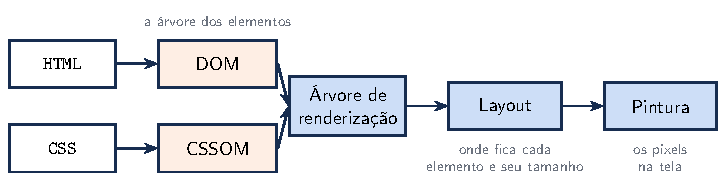
\includegraphics[width=0.95\linewidth,keepaspectratio]{imagens/capitulo-01_renderizacao.pdf}
\end{center}

\begin{enumerate}
  \item O navegador lê o HTML e monta o \textbf{DOM} (\textit{Document Object Model}), uma árvore em que cada elemento da página é um nó, dentro do seu elemento ``pai''. É no DOM que o JavaScript mexe para mudar a página (Capítulo 9).
  \item Ao encontrar uma folha de estilo, ele a baixa e monta o \textbf{CSSOM}, a árvore das regras de estilo.
  \item Juntando as duas, ele monta a \textbf{árvore de renderização}, só com o que vai aparecer, e já com o estilo de cada elemento.
  \item No \textbf{layout}, ele calcula a posição e o tamanho de cada elemento, de acordo com a largura da tela.
  \item Na \textbf{pintura}, ele desenha os pixels: textos, cores, bordas e imagens.
\end{enumerate}

Esse caminho explica algumas práticas que você vai ver ao longo da apostila. Um \textit{script} comum interrompe a leitura do HTML até ser baixado e executado; com o atributo \texttt{defer}, ele é baixado em paralelo e só roda quando o HTML terminou de ser lido. E sempre que o JavaScript muda a página, o navegador refaz as etapas de layout e pintura das partes afetadas, o que tem um custo quando é feito muitas vezes seguidas.

\subsection{1.8 As ferramentas de trabalho}

Para desenvolver para a Web, bastam três ferramentas, todas gratuitas:

\begin{itemize}
  \item um \textbf{editor de código}. O mais usado é o \textbf{Visual Studio Code} (VS Code), da Microsoft, para Windows, Linux e macOS. Ele colore o código, completa as \textit{tags} enquanto você digita e mostra erros;
  \item um \textbf{navegador moderno}, como o Chrome, o Edge ou o Firefox, com as ferramentas de desenvolvedor;
  \item um \textbf{servidor local}, para abrir as páginas como elas seriam abertas na Web.
\end{itemize}

As \textbf{ferramentas de desenvolvedor} (\textit{DevTools}) abrem com a tecla \texttt{F12}, ou com o botão direito do mouse sobre a página, na opção \textbf{Inspecionar}. Três abas vão ser usadas o tempo todo:

\begin{center}
\begin{tabular}{@{}P{0.22\linewidth}P{0.68\linewidth}@{}}
\toprule
\rowcolor{headergray}
\tblheader{Aba} & \tblheader{Para que serve} \\
\midrule
\textbf{Elements} & mostra o DOM e o CSS de cada elemento; dá para alterar os dois ali mesmo e ver o efeito na hora, sem mexer nos arquivos \\
\rowcolor{rowgray} \textbf{Console} & mostra os erros do JavaScript e permite executar comandos \\
\textbf{Network} & lista cada pedido feito pela página, com o método, o status, o tipo e o tempo \\
\bottomrule
\end{tabular}
\end{center}

Uma página pode ser aberta com um duplo clique no arquivo, e o endereço passa a começar com \texttt{file://}. Para as primeiras páginas, isso funciona, mas alguns recursos, como os pedidos do Capítulo 10, só funcionam quando a página é servida por HTTP. O jeito mais simples de ter um servidor no seu computador é a extensão \textbf{Live Server} do VS Code: com ela instalada, o botão \textbf{Go Live}, na barra inferior, abre a página no navegador e a recarrega a cada arquivo salvo. Quem já tem o Node.js instalado tem outra opção, sem extensão nenhuma, digitando no terminal, dentro da pasta do site:

\begin{codigo}
\begin{Verbatim}[breaklines=true, breaksymbolleft={}, fontsize=\footnotesize]
$ npx serve
 INFO  Accepting connections at http://localhost:3000
\end{Verbatim}
\end{codigo}

\subsection{1.9 A primeira página}

Crie uma pasta chamada \texttt{primeira-pagina} e, dentro dela, três arquivos. O primeiro é o HTML, com o conteúdo:

\begin{codigo}
\begin{Verbatim}[breaklines=true, breaksymbolleft={}, fontsize=\footnotesize]
<!DOCTYPE html>
<html lang="pt-BR">
<head>
  <meta charset="UTF-8">
  <meta name="viewport"
        content="width=device-width, initial-scale=1">
  <title>Minha primeira página</title>
  <link rel="stylesheet" href="estilo.css">
  <script src="script.js" defer></script>
</head>
<body>
  <h1>Olá, Web!</h1>
  <p>Esta página tem três arquivos: HTML, CSS e JavaScript.</p>
  <button type="button" id="botao">Clique aqui</button>
  <p id="mensagem"></p>
</body>
</html>
\end{Verbatim}
\end{codigo}

As linhas antes do \texttt{<body>} são o ``cabeçalho'' do documento, com informações para o navegador: o idioma, a codificação dos caracteres, o título que aparece na aba e os arquivos de estilo e de \textit{script} usados. Cada uma delas é explicada no Capítulo 2. O conteúdo visível fica dentro do \texttt{<body>}: um título, um parágrafo, um botão e um parágrafo vazio, que vai receber uma mensagem. O segundo arquivo, \texttt{estilo.css}, define a aparência:

\begin{codigo}
\begin{Verbatim}[breaklines=true, breaksymbolleft={}, fontsize=\footnotesize]
body {
  font-family: system-ui, sans-serif;
  max-width: 40rem;
  margin: 2rem auto;
  padding: 0 1rem;
}

h1 {
  color: #24124f;
}

button {
  padding: 0.5rem 1rem;
  cursor: pointer;
}
\end{Verbatim}
\end{codigo}

E o terceiro, \texttt{script.js}, dá vida ao botão:

\begin{codigo}
\begin{Verbatim}[breaklines=true, breaksymbolleft={}, fontsize=\footnotesize]
const botao = document.querySelector("#botao");
const mensagem = document.querySelector("#mensagem");

botao.addEventListener("click", () => {
  mensagem.textContent = "O JavaScript respondeu ao clique!";
});
\end{Verbatim}
\end{codigo}

O JavaScript procura o botão e o parágrafo vazio pelos seus \texttt{id}, e, a cada clique no botão, escreve uma frase no parágrafo. Abra a página com o Live Server, ou com o \texttt{npx serve}, e clique no botão:

\begin{center}

\includegraphics[width=0.85\linewidth,keepaspectratio]{imagens/capitulo-01_primeira-pagina.png}
\end{center}

Na aba Network das ferramentas de desenvolvedor, recarregue a página. A lista mostra os três pedidos que o navegador fez, um para cada arquivo, cada um com o seu tipo:

\begin{codigo}
\begin{Verbatim}[breaklines=true, breaksymbolleft={}, fontsize=\footnotesize]
GET /            200  text/html
GET /estilo.css  200  text/css
GET /script.js   200  text/javascript
\end{Verbatim}
\end{codigo}

O primeiro pedido, para \texttt{/}, devolveu o \texttt{index.html}: quando o caminho é uma pasta, os servidores procuram, por convenção, um arquivo com esse nome dentro dela. Os outros dois foram feitos porque o HTML os citou. Talvez apareça também um quarto pedido, para \texttt{/favicon.ico}, com status \texttt{404}, e um erro no Console: o navegador procura sozinho o ícone que aparece na aba, e a página ainda não tem um. Esse erro é inofensivo, e o Capítulo 2 mostra como declarar o ícone. Se você errar o nome de um arquivo, como \texttt{estilos.css} em vez de \texttt{estilo.css}, a página aparece sem estilo, e a aba Network mostra o pedido com o status \texttt{404}: é o primeiro lugar a olhar quando algo não carrega.

Por fim, uma página pode estar ``funcionando'' na tela e, mesmo assim, ter erros que um navegador perdoa e outro não. O \textbf{validador do W3C} (\texttt{validator.w3.org}) confere o HTML contra o padrão. Esta página foi conferida com ele e com o \texttt{html-validate}, outra ferramenta de validação, que acusou um detalhe na primeira versão: o \texttt{<button>} estava sem o atributo \texttt{type}. Sem ele, um botão dentro de um formulário envia o formulário ao ser clicado, o que nem sempre é o desejado; por isso a página declara \texttt{type="button"}, assunto do Capítulo 3.

\subsection{Erros Comuns}

\begin{itemize}
  \item \textbf{Confundir a Internet com a Web.} A Internet é a rede; a Web é um dos serviços que funcionam sobre ela.
  \item \textbf{Achar que o HTML é uma linguagem de programação.} Ele descreve o conteúdo; quem programa o comportamento é o JavaScript.
  \item \textbf{Errar o nome ou a pasta de um arquivo citado no HTML.} O navegador recebe um \texttt{404}, e a página aparece sem estilo ou sem \textit{script}. Confira a aba Network.
  \item \textbf{Misturar as três linguagens em um arquivo só.} Estilo e \textit{script} espalhados no HTML tornam qualquer mudança trabalhosa. Separe cada um no seu arquivo.
  \item \textbf{Esquecer o \texttt{defer} no \textit{script} do \texttt{<head>}.} O \textit{script} roda antes de o HTML existir, e o \texttt{querySelector} não encontra o elemento.
  \item \textbf{Testar só abrindo o arquivo com duplo clique.} Alguns recursos só funcionam com a página servida por HTTP. Use um servidor local.
  \item \textbf{Ignorar o Console.} Um erro de JavaScript costuma estar escrito lá, com o arquivo e a linha.
\end{itemize}
